\section{Framework Aspectual para aplicaciones de escritorio orientado a tareas}
\label{sec:framework_aspectual}

Los frameworks [y] pueden reducir los costos de desarrollo ya que permiten a los desarrolladores reusar experiencias previas en la resolución de problemas en los niveles de diseño e implementación del software. Investigaciones anteriores han demostrado que se pueden lograr altos niveles de reutilización del software a través del uso de frameworks ya que capturan aspectos comunes de una familia de aplicaciones. 
El esquema de la Fig.\ref{fig:fig2} ilustra de manera general la aplicación del framework desarrollado. El objetivo del framework es proveer mecanismos que posibiliten la evaluación de usabilidad automática aplicando el modelo presentado en la Sección~\ref{sec:eval_usabilidad}. Para diferentes aplicaciones de escritorio se proporciona un conjunto de módulos (clases-aspectos) que mediante la especialización de ciertos aspectos abstractos permiten reusar el diseño e implementación para calcular métricas y obtener información de la eficiencia, efectividad y satisfacción de las tareas de usuario.

%insertar fig2.png
\begin{figure*}[ht!]
	\centering
	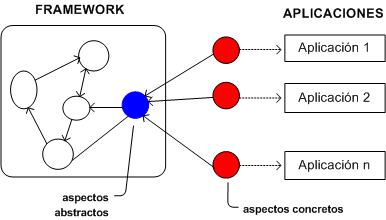
\includegraphics[scale=1]{figs/fig2.png}
	\caption{\label{fig:fig2} Esquema general del framework.}
\end{figure*}


\subsection{Requerimientos}
\label{subsec:requerimientos}
El framework ha sido construido desde cero aplicando un proceso iterativo de sucesivos refinamientos. Inicialmente se estableció el concepto y alcance de tarea. Definitivamente la tarea es un conjunto de acciones \colorbox{green}{significativas para el usuario} que ocurre-sucede durante la ejecución de la aplicación. Sin embargo, este concepto no está representado como entidad del sistema, por ser un concepto subyacente y subjetivo. La tarea entonces debe ser representada en el framework, resultando esta abstracción de una relevancia central dado que todo el framework requiere mantener relaciones e interacciones que son dependientes de la misma. Desde esta visión una  tarea es una entidad subyacente a la aplicación que requiere encapsular un conjunto de estados y comportamiento interno,  puesto que realiza una o más operaciones y provee un comportamiento global para lograr el objetivo específico. Por lo cual, cualquier y toda tarea podrá ser relacionada con algún evento del sistema que establece su inicio y también con otro evento que indica su finalización. Una tarea podrá ser instanciada diversas veces en la misma o distintas ejecuciones de la aplicación (sesiones), cada instancia deberá ser identificable, ya que comporta diferentes valores para los estados descriptores. 

A partir del planteo de un escenario general y abstracto se ha procedido a identificar el conjunto de eventos que desencadenan las acciones que ejecutará y/o controlará el framework y el tipo de módulo (clase o aspecto) del framework que será responsable de ejecutar la función correspondiente (Tabla\ref{tab:tab1}).  Los  eventos se clasifican en dos categorías según su origen. Los eventos de la aplicación (se ha producido un error mientras se ejecutaba la tarea) o los eventos pueden ser activados  por el mismo framework (se instancia una tarea). Asimismo un evento puede desencadenar una o más acciones, las cuales pueden ser llevadas a cabo por distintos módulos. 

%insert table1
% \usepackage{multirow}
\begin{table}[h]
\centering
\caption{Eventos-Acciones-Módulos}
\label{tab:tab1}
\begin{tabular}{|l|l|l|l|l|}
\hline
\multicolumn{2}{|c|}{Evento}                                                                                            & \multicolumn{2}{c|}{Acciones/Responsabilidad}                                              & \multicolumn{1}{c|}{Módulo} \\ \hline
\multirow{2}{*}{E1} & \multirow{2}{*}{\begin{tabular}[c]{@{}l@{}}Ejecución del \\ inicio de una tarea (D)\end{tabular}} & A1  & Interceptar inicio de una tarea                                                      & \multirow{2}{*}{Aspecto}    \\ \cline{3-4}
                    &                                                                                                   & A2  & Instanciar una tarea                                                                 &                             \\ \hline
\multirow{2}{*}{E2} & \multirow{2}{*}{Instanciar Tarea (F)}                                                             & A3  & Registrar inicio de la tarea                                                         & Clase                       \\ \cline{3-5} 
                    &                                                                                                   & A4  & Logging inicio de la tarea                                                           & Aspecto                     \\ \hline
\multirow{2}{*}{E3} & \multirow{2}{*}{\begin{tabular}[c]{@{}l@{}}Ejecución del \\ fin de una tarea (D)\end{tabular}}    & A5  & Interceptar el fin de una tarea                                                      & \multirow{2}{*}{Aspecto}    \\ \cline{3-4}
                    &                                                                                                   & A6  & Ordenar el fin de la tarea                                                           &                             \\ \hline
\multirow{3}{*}{E4} & \multirow{3}{*}{Finalizar la tarea (F)}                                                           & A10 & Registrar fin de la tarea                                                            & Clase                       \\ \cline{3-5} 
                    &                                                                                                   & A11 & \begin{tabular}[c]{@{}l@{}}Proporcionar el \\ Cuestionario Satisfacción\end{tabular} & \multirow{2}{*}{Aspecto}    \\ \cline{3-4}
                    &                                                                                                   & A12 & Logging Datos del fin de la tarea                                                    &                             \\ \hline
\multirow{3}{*}{E5} & \multirow{3}{*}{Seproduce un error (D)}                                                           & A7  & Identificar el error                                                                 & \multirow{2}{*}{Aspecto}    \\ \cline{3-4}
                    &                                                                                                   & A8  & Logging errores                                                                      &                             \\ \cline{3-5} 
                    &                                                                                                   & A9  & Contabilizar error                                                                   & Clase                       \\ \hline
\end{tabular}
\end{table}

Los eventos E1 y E3, originados en el dominio (D), permiten identificar, delimitar y hacer el seguimiento de la tarea durante su tiempo de vida (ejecución), lo que implica que debidamente generarán las acciones de instanciación (A1-A2) y finalización(A5-A6), estas acciones serán llevadas a cabo por un aspecto. Al instanciar una tarea (E2) es necesario comenzar a registrar los datos (A3) que serán necesarios para el cálculo de métricas (duración) y accionar el log de la tarea (A4). En esta sucesión de eventos y acciones, el framework condiciona una cantidad de acciones a eventos internos que están supeditados a los cambios de la tarea. Esta premisa hace a los módulos del framework más independientes del dominio.

\subsection{Diseño e Implementación}
\label{subsec:disenio_e_implementacion}

En la Figura\ref{fig:fig3} se presenta el diseño del framework, la implementación está desarrollada en Java y AspectJ. La clase Task constituye el núcleo del framework, dado que mantiene diversas relaciones con los restantes módulos. Los aspectos tienen un rol preponderante, ya que son necesarios para conectar la tarea con la aplicación y para comunicarla con otros servicios del framework (logging). El aspecto TaskConnect conecta a la tarea con los correspondientes eventos de inicio y finalización y realiza las acciones de crear la instancia de la Task y ordenar su finalización. El aspecto TaskError intercepta los errores que se producen en la ejecución de la tarea creada por TaskConnect y el aspecto TaskSatisfaction facilita un formulario que permite registrar la información subjetiva cuando la tarea ha sido finalizada. El aspecto TaskLog registra el logging de las tareas, cuando estas se crean, finalizan o generan otros eventos, de manera que es dependiente de la tarea y no de la aplicación. 

%insertar fig3
\begin{figure*}[ht!]
	\centering
	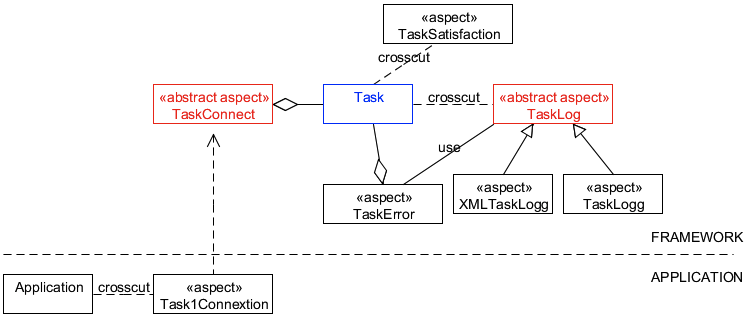
\includegraphics[scale=1]{figs/fig3.png}
	\caption{\label{fig:fig3}  Diseño del framework.}
\end{figure*}

A continuación se presenta los principales detalles del diseño interno e implementación de los módulos del framework. Cómo se mencionó la clase Task representa una tarea del usuario. Tiene diversos estados que permiten calcular posteriormente métricas o que van acumulando los valores de las mismas. Estos estados son inicializados en su instanciación. El atributo init se inicializa con la hora del sistema y el atributo complete con el valor falso. Estos dos atributos serán posteriormente actualizados por el método finalize (cuando la tarea finaliza) y usados para calcular el tiempo (eficiencia de la tarea) y si se ha completado (efectividad de la tarea). Para cada atributo que permite contabilizar errores como los atributos relacionados a la satisfacción existen métodos que permiten su correcta actualización. 

\begin{verbatim}
class Task  {
  private String id,
  private Time init, end;
  private boolean complete;
  private int #exception, sat1, sat2, sat3;
  Task(..){
     // inicialización de estados}
   ..
   …
  finalize()
    {// actualización de estados }
}

\end{verbatim}

El aspecto abstracto TaskConnect conecta la tarea con la aplicación. Dos pointcuts abstractos startTask y endTask son necesarios para definir los join-points (clase y método del dominio)  en los cuales comienza y finaliza cada tarea. Estos deberán ser definidos en un aspecto concreto por el desarrollador, que deberá crear un subaspecto por cada tarea de usuario distinta que pretenda evaluar. TaskConnect  tiene por atributo una tarea, (objeto  de tipo Task) que es instanciado por dicho aspecto cuando el pointcut startTask es activado y se ejecuta el aviso asociado, lo cual ocurre antes de que cada tarea inicie. De manera similar, este aspecto ordena la finalización de la tarea cuando luego que se activa el pointcut endTask, por medio del aviso asociado, se invoca al método.  

\begin{verbatim}
abstract aspect TaskConnect {
   private String idTask;
   private Task t;
   abstract pointcut starTask; 
   abstract pointcut endTask;

   before() : initTask();
   {  this.setTask();
      t = new Task(idTask);}
   after() : endTask()
   { t.finalize(); }
}
\end{verbatim}

El aspecto TaskError tiene por objeto interceptar los errores que se producen durante la ejecución de una tarea y ordenar la actualización de los acumuladores correspondientes de la tarea. El aspecto mantiene una referencia a la tarea instanciada, por medio del pointcut beginning y el atributo monitored\_task. Luego por cada tipo de error que se registra, se define un pointcut y advice. Tal es el caso del pointcut exception, cuyo objetivo es interceptar las excepciones que se producen mientras la tarea se ejecuta. Para ello es necesario especificar varias condiciones, que permiten delimitar al conjunto de excepciones que se producen. Estas restricciones debido a que también son necesarias para la intercepción de otros tipos errores se especifican en forma aislada e individual en los pointcuts condition\_1, condition\_2 y condition\_3. Luego en el pointcut exception se combinan con el descriptor de pointcut más específico, para este caso, handler. El advice asociado, primero actualiza el contador de excepciones de la tarea y luego ordena el log del error, operación que realiza el aspecto TaskLog. 

\begin{verbatim}
aspect TaskError {
  Task monitored_task=null;
  pointcut inicialization():    
               initialization(Task.new(String));

  pointcut beginning(Task t):inicialization()&&this(t);
  after(Task t): beginning(t)
    {monitored_task=t;} 

  pointcut condition_1():!cflow(adviceexecution)
  pointcut condition_2():!cflow(inicialization) 
  pointcut condition_3():if ((monitored_task!=null)&&
                            (!monitored_task.isComplete()))
  pointcut exception(Throwable e): 
                handler(Throwable+) && args(e)
                && condition_1() && condition_2()
                && condition_3()

  before(Throwable e): exception(e) {
     // actualizar monitored_task;
     TaskLog.aspectof().logException(e);
  }
}

\end{verbatim}

Cuando se produce la finalización de una tarea, (el método finalize de Task es invocado por el aspecto TaskConnect), el aspecto TaskSatisfaction proporciona un cuestionario que permite obtener información subjetiva del usuario relacionada a la dimensión satisfacción. Este formulario es muy simple, permite al usuario elegir un valor entre 1 y 5 para cada una de las 3 preguntas que se muestran en pantalla. 

\begin{verbatim}
aspect TaskSatisfaction {
   pointcut satisfaction(Task t):
        execution(void Task.finalize(..))&&this(t);	
   before(Task t): satisfaction (t) {
	// desplegar cuestionario 
       // obtener datos ingresados por el usuario.
	// actualizar atrubutos sat1..de t
   return;}
}

\end{verbatim}

Finalmente el aspecto TaskLog  realiza el logging de la tarea en diversos momentos. Es una aspecto abstracto debido a que el log puede realizarse en diversos formatos (texto / xml / base de datos / consola). Los pointcut están definidos de manera concreta, ya que este aspecto está supeditado por completo a los cambios en la tarea.  

\begin{verbatim}
abstract aspect TaskLog {
   abstract void logException() // log de excepciones
   abstract void logTask() {//}
   pointcut logSart(Task): call Task.new(..) && target(t);
   pointcut logEnd(Task): call Task.finalize(..) && target(t);
   after() : logStart()
   { logTask(t);}
   after() : logEnd()
   { logTask(t);}
}

\end{verbatim}

El diseño e implementación de los módulos del framework se ha apoyado en distintos patrones de diseño aspectuales [xx]. Por ejemplo, en el caso de TaskConnect se aplicaron los patrones Abstract Pointcut y Template Advice, en TaskError se aplicó el patrón Composite Pointcut y en TaskLog se aplicó el patrón Template Advice.